\section{Équilibre et optimum}

Les prix d'équilibre sont déterminés par les conditions d'égalité de l'offre et de la demande sur chaque marché. On égalise donc la demande d'un bien à son offre $D_1=O_1$.\\
Cas particulier:\\

Si sur les différents marchés les préférences sont \textbf{les mêmes} et les dotations sont \textbf{proportionnelles} (par exemple $dotation_1 +dotation_2=constante$ alors il n'y aura pas d'échange à l'équilibre en autarcie. En effet les TMS des deux marchés seront égaux ce qui veut dire qu'il n'y a aucun échange rentable pour les deux marchés.\\

De plus si les fonctions de demande sont linéaires et identiques, on peut les exprimer en fonction du pourcentage de la richesse totale:
$$
c_i^j=\frac{W_j}{W_T}\Omega_i
$$
En effet 
$$
c_i^j= \lambda W_j \Leftrightarrow \frac{c_i^j}{\Omega_i}=\frac{\lambda W_j}{\lambda W_T}
$$



\textbf{Loi de Walras}: \textit{Si des N marchés, N-1 sont en équilibre alors le $N^{\text{ème}}$ est en équilibre}

\subsection{Optimum de Pareto}

Un optimum de pareto se définie comme une allocation des biens \textbf{ne permettant pas les échanges mutuellement avantageux}. Le programme se définit comme suit:
$$
\left\{
\begin{array}{cc}
 max_{C_i}U= & F(C_1,..,C_n)  \\
 sc: & \\
 & \sum_i p_i C_i \leq W \ \forall i \in \{ 1,..n .\}\\
 & U_j \leq \bar{U} \ \forall i \in \{ 1,..n .\}
\end{array} 
\right.
$$

On obtiens comme conditions menant à l'optimalité:
\begin{itemize}
\item $TMS_{i,j}^{k}=TMS_{i,j}^{u}$ égalité des TMS, donc plus aucun échange n'est mutuellement profitable.
\item Saturation des contraintes budgétaires si U croissante en $C_1,..,C_n$
\end{itemize}


\subsection{La boite d'Edgeworth}

Cette une façon graphique d'analyser les problèmes d'équilibres. Elle représente les biens des 2 agents sur les marchés, ces biens étant limités à l'offre totale de chacun d'entre eux. Elle nous permet aussi d'observer graphiquement la courbe des contrats, (ensemble des optimums de Pareto) qui se constitue de l'ensemble des points de tangence entre les courbes d'indifférences des 2 agents.
\newpage
\begin{figure}[h]
\begin{center}
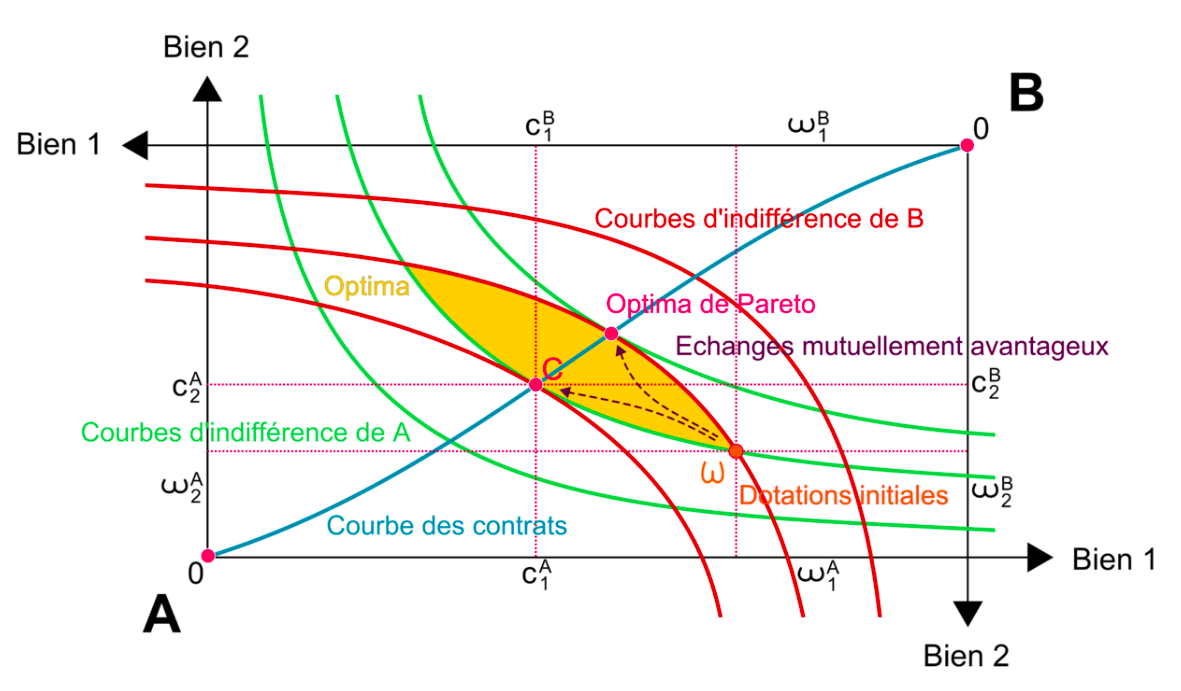
\includegraphics[scale=0.3]{./img/IM2}
\caption{La boite d'Edgeworth}
\end{center}
\end{figure}